\documentclass[reqno]{article}

\usepackage{fullpage}
\usepackage{eufrak}
\usepackage{listings}
\usepackage{color}
\usepackage{xcolor}
\usepackage{enumitem}


% \usepackage{nth}
\usepackage{amsthm,amsmath,amsfonts,amssymb}


%formatting
\usepackage[left=2cm,right=2cm,top=2cm,bottom=2cm,bindingoffset=0cm]{geometry}
\renewcommand{\baselinestretch}{1.2}
\sloppy

% Languages, fonts and symbols
\usepackage[english,russian]{babel}
\usepackage[T1,T2A]{fontenc}
\usepackage[utf8]{inputenc}
\usepackage{titlesec}

\usepackage{amsmath}

\usepackage{array}

\usepackage{graphicx}
\graphicspath{{images/}} 
\DeclareGraphicsExtensions{.pdf,.png,.jpg}

\usepackage{subcaption}

\usepackage{amssymb}

\usepackage{listings}

\usepackage{float}

\usepackage{dsfont}

\usepackage{ragged2e}

\usepackage{tabularx}

\usepackage{footmisc}

%\usepackage{algorithm}
\usepackage[ruled,vlined]{algorithm2e}

\SetKwInput{KwInput}{Input}                % Set the Input
\SetKwInput{KwOutput}{Output}              % set the Output


% tikz graphics
% Для коммутативных диаграмм.
\usepackage{tikz}
\usetikzlibrary{arrows,shapes}
\tikzstyle{vertex}=[circle,fill=black,minimum size=3pt,inner sep=0pt]
\tikzstyle{edge} = [draw,thick,-]

\usepackage{tikz-cd}

\usetikzlibrary{quotes,babel,angles}


% Теоремы и прочее
\renewcommand\qedsymbol{$\square$}

\theoremstyle{definition}
\newtheorem*{nb}{Замечание}

\theoremstyle{definition}
\newtheorem*{sol}{Решение}

\theoremstyle{definition}
\newtheorem*{exmp}{Пример}

\theoremstyle{definition}
\newtheorem*{exmps}{Примеры}

\theoremstyle{definition}
\newtheorem{exc}{Упражнение}[section]

\theoremstyle{definition}
\newtheorem{thm}{Теорема}[section]

\theoremstyle{definition}
\newtheorem*{defi}{Определение}

\theoremstyle{definition}
\newtheorem{coll}{Следствие}[section]

\theoremstyle{definition}
\newtheorem{state}{Утверждение}[section]


%Content as links

\usepackage[hidelinks]{hyperref}
\hypersetup{
	colorlinks,
	citecolor=black,
	filecolor=black,
	linkcolor=black,
	urlcolor=black
}


% Title
\title{Математические модели микро- и макроэкономики.\\ Лекции.\\ ЧЕРНОВИК}
\author{Лектор: Мозговая К.А.\\ \\ Авторы конспекта: \\ Курмазов Ф.А.\\ Кривогорницына В.А.}
\date{\today}


% New Symbols
\newcommand*{\divby}{\mathrel{\rotatebox{90}{$\hskip-1pt.{}.{}.$}}}%

\begin{document}
	
	\setlength{\parindent}{0pt}
	\setlength{\parskip}{0.3em}
	
	\maketitle
	
	\tableofcontents
	\newpage
	
	\section{Лекция 1.}
	\subsection{Человеческий капитал}
	Человеческий капитал - экстерналия. Абсолютно невидимая вещь, которая приносит пользу обществу. То есть накопление нами знаний, умений, навыков, труда, невидимым образом повышает уровень развития общества.
	
	\begin{defi}
		Человеческий капитал — совокупность знаний, умений, навыков (существующие у каждого индивида), которые используются для удовлетворения многообразных потребностей общества в целом.
	\end{defi}
	
	Человеческий капитал так же, как и физический, можно считать средством производства. Инвестиции в него приносят выгоду для общества в целом. И имеет место быть теория о том, что чем больше человеческого капитала, тем проще его накапливать. 
	
	В конце 20 века, в частности с развитием математических дисциплин (в том числе анализа данных, эконометрики...), экономисты пришли к выводу, что человеческий капитал, наряду с физическим, является неотъемлемым фактором современного экономического роста.
	
	С того момента в понятие человеческий капитал стали вносить также \textbf{здоровье, жизненный опыт и заботу о распорядке своего дня}. Ведь нанимать на работу здорового развитого человека лучше и выгоднее, чем нанимать того, на которого в будущем необходимо будет тратить деньги, чтобы лечить.
	
	Сейчас экономическая политика большинства развитых стран направлена увеличение инвестиций в человеческий капитал. Так как он сильно влияет на уровень выпуска в экономике и на темп его роста. 
	
	\subsection{Экономический рост}\label{sec:1.2}
	
	\begin{defi}
		Экономический рост - долгосрочная тенденция увеличения реального ВВП на душу населения в государстве.
	\end{defi}
	
	Чем выше темп экономического роста, тем выше уровень жизни в государстве. Калдор выделял \textbf{шесть факторов, которые должна включать в себя любая модель роста}:
	
	\begin{itemize}
		\item ВВП и производительность труда растут с течением времени;
		\item Величина физического капитала на одного рабочего растет во времени;
		\item Реальная ставка процента почти не меняется во времени (в развитых странах);
		\item Отношение запаса физического капитала к ВВП приблизительно постоянно;
		\item Доли заработных плат и дохода на капитал в структуре НД примерно постоянны;
		\item Темп роста выпуска на одного рабочего значительно отличается в разных странах.
	\end{itemize}
	
	В дальнейшем последовала колоссальная критика вышеперечисленных принципов. Тома Пикетти выпустил книгу "Капитал в XXI веке", в которой критиковалось отношение капитала к выпуску и критиковалась доля дохода на капитал. Он говорил, что доля должна демонстрировать всегда тенденцию к увеличению, а не к постоянству. Критика заключалась в том, что если доля всегда имела постоянный темп, то как выпуск на душу населения может расти, что тогда двигает этот рост становится не понятно.
	
	Несмотря на это, именно вышеперечисленные 6 постулатов Калдора заложили основу развития модели Солоу.
	
	\subsection{Модель Солоу}
	Модель Солоу -- модель экзогенного экономического роста. Она объясняет долгосрочный рост в экономике исключительно внешними факторами.
	
	Мы имеем выпуск, который задается неоклассической производственной функцией, зависящей от двух факторов производства (труда и капитала). 
	
	$$Y_t=F(K_t,L_t)$$
	
	\textbf{Свойства $F(K,L)$}:
	\begin{enumerate}
		\item Постоянная отдача от масштаба 
		$$F(\lambda K, \lambda L) = \lambda F(K, L)$$
		
		\item Положительная и уменьшающаяся отдача от факторов производства
		$$\forall K,L > 0, F'_K (K, L) > 0, F'_L (K, L) > 0; F''_K (K, L) < 0, F''_L (K, L) < 0 $$
		$F'_K (K, L), F'_L (K, L)$ - предельная производительность труда и капитала соответственно.
		
		Т.е. мы не можем использовать $\infty$ - много какого-либо фактора производства, так как в какой-то момент увеличение этого фактора на единицу будет приносить снижение выпуска.
		
		Также мы не можем увеличивать один фактор, не изменяя другой (нам не нужно 100 ножек для стола, если крышек у нас всего 10).
		
		\item Условия Инады:
		\begin{itemize}
			\item Все факторы нужны для производства.
			$$\lim_{K \rightarrow 0} F'_K (K, L) = \lim_{L \rightarrow 0} F'_L (K, L) = \infty$$
			
			Мы не можем использовать только станки, оборудование...(капитал) и не использовать людей (труд). И наоборот.
			
			\item Выпуск растет при росте факторов производства.
			$$\lim_{K \rightarrow \infty} F'_K (K, L) = \lim_{L \rightarrow \infty} F'_L (K, L) = 0$$
			
			Чем больше мы используем труда и капитала, тем больше выпуск.
		\end{itemize}
	\end{enumerate}
	
	Также можно перейти к другой записи модели, пронормировав весь выпуск по количеству занятой рабочей силы.
	
	\textbf{Капиталовооруженность труда}, т.е. величина капитала на одного рабочего $$k=\frac{K}{L}$$
	
	Соответственно у нас будет выпуск зависеть от капиталовооруженности: $f(k)$.
	
	Формулировка модели в величинах на душу населения удобна тем, что \emph{исключает зависимость от масштаба}: при постоянной капиталовооруженности $k$ увеличение или уменьшение населения (рабочей силы) не влияет на производительность.
	
	\textbf{"Репрезентативный" потребитель} - общество в целом. Мы знаем его поведение, предпочтения, рабочую силу и доход (нам не важно как он сформировался).
	
	В модели Солоу все потребители (агенты) друг от друга не отличаются, поэтому \emph{население можно считать единым "репрезентативным" потребителем}. Весь произведенный в периоде $t$ продукт после выплаты дохода на капитал и заработной платы оказывается сосредоточен у "репрезентативного" потребителя.
	
	Весь выпуск, который сосредотачивается у "репрезентативного" потребителя, приведен в некотором стоимостном выражении. Этот выпуск в денежном эквиваленте делится на потребление "репрезентативного" потребителя и его инвестиции.
	
	\begin{equation}\label{eq:1.3.1}
		Y_t = C_t + I_t
	\end{equation}
	
	Т.е. в каждый момент времени потребитель принимает решение, сколько он хочет потреблять (тратить деньги на товары, услуги, развлечения...), а сколько инвестировать (вложение в банк, ценные бумаги или под матрас... То есть то, что сейчас не тратится на потребление).
	
	В двухфакторной модели инвестиции можно назвать сбережениями.\bigskip
	
	На что направлены инвестиции? 
	
	Если посмотреть весь процесс, то наши сбережения попадают в банк, а впоследствии фирма берет кредит этого банка на развитие производства. Соответственно эти инвестиции формируют капитал:
	
	\begin{equation}\label{eq:1.3.2}
		K_{t+1} = (1 - \mu) K_t + I_t
	\end{equation}
	
	То есть капитал в каждый следующий период времени - это тот фактор производства, на который ориентируется фирма для того чтобы производить больше выпуска.
	
	Деньги от ``репрезентативного'' потребителя, которые не тратятся на потребление, направляются на развитие фирмы.  \emph{Соответственно уравнение \ref{eq:1.3.1} и \ref{eq:1.3.2} показывают, то, как много будет накапливаться капитала, для того чтобы увеличивался выпуск фирмы}. Если бы капитал не подлежал износу, то все деньги шли на развитие фирмы, но так как все наше оборудование изнашивается, это необходимо учесть (первое слагаемое уравнения \ref{eq:1.3.2}).
	
	Также у нас есть труд (вся рабочая сила, задействованная в производстве), который не является константой. Население растет, соответственно, вся рабочая сила изменяется из периода в период. 
	\begin{equation}\label{eq:1.3.3}
		L_{t+1} = (1 + n) L_t
	\end{equation}
	где $n$ - темп роста населения
	
	Таким образом состояние экономики меняется из периода в период. Выпуск зависит от потребления в текущий период времени; от капитала, который мы хотим направить на развитие производства в будущий период времени и от того, сколько сейчас людей задействовано в производстве. 
	
	Соответственно наше решение сегодня (сколько потреблять, а сколько инвестировать) влияет на выпуск завтра. И темп роста населения сегодня влияет на то, сколько людей будет задействовано в развитии выпуска завтра. 
	
	Отсюда получаем, что вся модель является \emph{динамической}.\bigskip
	
	В моделях роста интересным является тот факт, как же выпуск $Y_t$ распределяется между потреблением $C_t$ и инвестициями $I_t$.
	
	Модель Солоу основана на самом простом предположении, что деление выпуска на потребление и валовые инвестиции осуществляется с помощью заданной извне и не меняющейся с течением времени нормы сбережения $s$ $(0 < s < 1)$. 
	
	$$I_t = s Y_t$$
	$$K_{t+1} = (1 - \mu) K_t + s F(K_t, L_t)$$
	$$\frac{K_{t+1}}{L_{t+1}} = (1 - \mu) \frac{K_t}{L_{t+1}} + \frac{s F(K_t, L_t)}{L_{t+1}}$$
	
	Таким образом, мы получаем уравнение, задающее динамику в модели Солоу:
	
	\begin{equation}\label{eq:1.3.4}
		(1 + n) k_{t + 1} = (1 - \mu) k_t + s f(k_t)
	\end{equation}
	
	Таким образом, если мы будем знать $k_0$, то мы будем знать весь выпуск из периода в период.
	
	Так как выпуск на душу населения задается:
	$$y_t = \frac{Y_t}{L_t} = f(k_t)$$
	Можно однозначно указать значения выпуска на душу населения $(y_t)_{t=0,1,\dots }$ и потребление на душу населения $(c_t)_{t=0,1,\dots}$ \bigskip
	
	\textbf{Траектория в модели Солоу} (исходящая из начального состояния $k_0$) - последовательность капиталовооруженностей и удельных потреблений $(k_t, c_t)_{t=0,1,\dots}$. Т.е. как менялась капиталовооруженность из периода в период.
	
	При отображении на графике мы будем видеть две независимые функции
	
	\begin{figure}[h!]
		\centering
		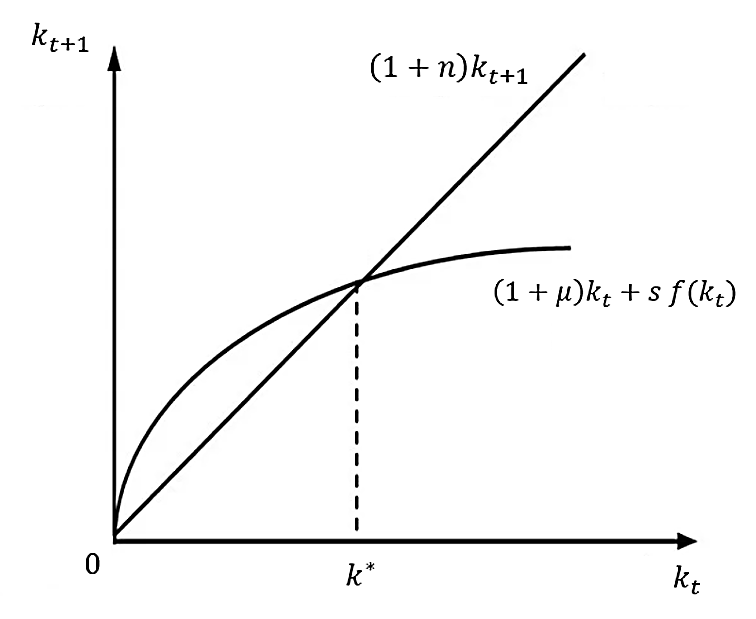
\includegraphics[width=0.35\textwidth]{Cтационарное_состояние_Солоу}
		\caption{Cтационарное состояние Солоу}
	\end{figure}
	
	где $k^*$ - это  точка стационарного состояния в системе. После неё не будет наблюдаться такого большого роста в экономике, который был до.
	
	Точка стационарного состояния в системе - некоторый уровень капиталовооруженности и потребления на душу населения, который не меняется с течением времени ($k^* = k_0^* = \dots = k_t^* = \dots; c^* = c_0^* = \dots = c_t^* = \dots$). 
	
	Тогда $$(n + \mu) k^* = s f(k^*)$$
	
	$k^*=0$ удовлетворяет равенству, при этом в силу условий Инады для производственной функции выполняется $f'(0) > n + \mu$
	
	Из сходимости последовательности капиталовооруженностей следует сходимость выпуска на душу населения к своему стационарному значению $f(k_t) \rightarrow f(k^*)$, а потребления к $c^* = (1-s)f(k^*)$. То есть удельные величины стабилизируются со временем, и это является той точкой, в которую пытается прийти любая динамическая система. 
	
	\textbf{Устойчивое состояние в системе} - максимально возможный капитал, максимально возможное потребление, которое мы можем добиться в нашей системе, если мы абстрагируемся от того, что существует индекс времени.
	
	Это теоретическая конструкция, без которой мы не можем говорить, что происходит на конкретных данных и как анализируются конкретные данные, посвященные накоплению капитала, потребления или данные, которые публикуются, связанные с ВВП.\bigskip
	
	От переменных капиталовооруженности мы можем перейти к переменным, которые описывают запас капитала в валовом исчислении. Получается мы переходим от удельных величин к валовым, и говорим какой объем капитала или выпуска мы ожидаем из периода в период. 
	
	$$\lim_{t \rightarrow \infty} \frac{K_{t+1}}{K_t} = \lim_{t \rightarrow \infty} \frac{Y_{t+1}}{Y_t} = 1 + n$$
	
	Никакое изменение параметров модели не может повлиять на постоянство удельных величин в долгосрочном периоде. Получается, что модель Солоу без технического прогресса не объясняет, откуда в долгосрочном периоде возникает рост на душу населения.
	
	Изменения $s, n, \mu$ или параметров производственной функции могут оказывать влияние только на уровни удельных переменных в стационарном состоянии.
	
	И именно предпосылка о константности нормы сбережения вызвала наибольшую критику модели Солоу. Эта предпосылка считается уникальной в своем роде, так как являлась неким прорывом в изучении моделях роста; но также она крайне неправдоподобна, так как не может из периода в период на инвестиции уходить фиксированная часть. Потому что все меняется, и меняется сама по себе суть модели, так как на принятие решения какую часть выпуска мы хотим отправить на инвестиции являются внешние факторы. Внешние факторы - шоки, которые из периода в период разные, поэтому и s не может быть стационарной. У нас должно быть написано уравнение, связывающее инвестиции и выпуск, и оно должно зависеть от многих факторов.
	
	\subsection{Модель Солоу с техническим прогрессом}
	
	Солоу сам говорил, что в его модели всегда будет рост и берется он с некоторого остатка. То есть Солоу предполагал, что существует набор факторов, который влияет на экономику.
	
	Последующие модели стали включать в себя, наряду с запасом физического капитала ($K_t$) и количеством труда ($L_t$), также параметр технического прогресса($A_t$)
	
	$$Y_t = A_t F(K_t,L_t)$$
	
	\textbf{Остаток Солоу (темп роста совокупной производительности факторов)} для функции Кобба-Дугласа:
	$$g^A = g^Y - \alpha g^K - (1 - \alpha) g^L$$
	, где
	
	$g^A$ - темп роста совокупной производительности факторов,
	
	$g^Y$ - темп роста выпуска,
	
	$g^K, g^L$ - темпы выпуска факторов производства,
	
	$\alpha, (1 - \alpha)$ - эластичности выпуска по факторам производства.
	
	\subsection{Последующие модели}
	Холодная война в 1960 годах заставила США разрабатывать стратегию роста, которая затмила бы СССР(основанную на двух параметрах $K$ и $L$).
	
	Так Шульц предложил повысить гос. расходы на образование. Которые, по его мнению, дадут США не только преимущество в гонке, но и обогатят человеческие ресурсы в целом, что повысит ее производительность.
	
	Фридман был не согласен и с Шульцом, и считал, что вложение в индивида будет пустой тратой денег. Так как возможно этот человек не хочет трудиться на благо страны, а  заботится только о себе.
	
	Он был только за индивидуальную свободу в обществе и капиталистическое предпринимательство. Индивид сам должен решать какое образование получать, или какой заработной платы он достоин на основании своих базовых знаний. То есть Фридман отрицал необходимости выдачи кредитов на образование, при этом индивиды должны были стать частными предпринимателями. И страна должна нанимать на работу не индивидов, а только частных предпринимателей. Ведь перевод рабочих в разряд независимых предпринимателей может укрепить в экономике регрессивную тенденцию рабочих договоров, в случае котором все издержки найма переходят на работника.  
	
	Таким образом Фридман и Шульц доказали важность человеческого капитала, доказали его влияние на экономический рост.
	
	\begin{center}
		Некоторые выводы ученых о важности человеческого капитала:
	\end{center}
	
	\textbf{A.Smith}: 
	
	Навыки и умения, полученные работниками (например, в ходе обучения, тренировки) могут повысить экономическую ценность предприятия;\\
	
	\textbf{R.Nelson}: 
	
	Образованные люди совершают инновации, таким образом, образование ускоряет процесс развития технологий;\\
	
	\textbf{Z.Griliches}:
	
	Дальнейшее образовательное движение работника не может быть ограничено только "пулом" его прошлых способностей;\\
	
	\textbf{R.Lucas}: 
	
	Чем выше уровень людей, с которыми Вы работаете, тем больше Вы выучите и больших навыков приобретете.
	
	
	\newpage
	
	\section{Лекция 2.}
	
	\subsection{Организационные моменты.}
	
	КТ1 3 апреля, КТ2 где-то в мае.
	
	\subsection{Оптимизационные задачи.}
	
	\begin{exmp}
		$$\max_{x,y \in\mathds{R}_{\geq 0}} x$$
		$$\text{s.t.} y - (1 - x)^3 \leq 0$$
	\end{exmp}
	
	Способы решения:
	\begin{enumerate}
		\item Графический.
		\item Метод Лагранжа.
	\end{enumerate}
	
	Лагранжиан:
	$$\mathfrak{L}(x, y, \lambda, \mu_x, \mu_y) = x - \lambda(y - (1 - x)^3) + \mu_xx + \mu_yy$$
	
	\begin{thm}
		Условия Каруша-Куна-Такера:
		\begin{enumerate}
			\item $FOC[\bar{x}] = \frac{d\mathfrak{L}}{d\bar{x}} = \bar{0}$
			\item Условия дополняющей нежесткости. Все слагаемые лагранжа $= 0$.
			\item Ограничения задачи.
			\item $\bar{\lambda} \geq 0$
		\end{enumerate}
	\end{thm}
	
	Условия Каруша-Куна-Такера для примера:
	\begin{equation}
		\begin{cases}
			1 - 3\lambda(1 - x)^2 & = 0\\
			-\lambda + \mu_y& = 0\\
			\lambda(y - (1 - x)^3)& = 0\\
			\mu_xx & = 0\\
			\mu_yy & = 0\\
			y - (1-x)^3 &\leq 0\\
			y, x &\geq 0\\
			\lambda, \mu_x, \mu_y &\geq 0
		\end{cases}
	\end{equation}
	
	Решение задачи: $(x^*, y^*, \lambda^*, \mu_x^*, \mu_y^*)$.
	
	Приведенная в примере задача не решается с пом. теоремы Каруша-Куна-Такера, т.к. не выполняются условия Якоби.
	
	\begin{thm}
		\textcolor{red}{???}\textbf{Условие Якоби}: для любой точки, ранг матрицы Якоби системы активных ограничений $=$ количеству ограничений в ней.			
	\end{thm}
	
	\subsection{Модель потребительского выбора.}
	
	\begin{defi}
		\textbf{Задача потребительского выбора} -- требуется описать экономическую активность индивида связанную с выбором потребителем пакета потребляемых благ.
		
		Модель, описывающая потребительских выбор может учитывать: его частные интересы, его стремление выбрать лучшую стратегию.
	\end{defi}
	
	$X$ - \textbf{набор альтернатив} (множество в некотором пространстве).
	Чаще всего $X = \mathds{R}^L_{\geq 0 }$.
	
	\textbf{Вектор потребляемых благ} $x \in X$.
	
	\textbf{Множество потребляемых благ} $X\in \mathds{R}^L$.
	
	\textbf{Вектор цен} $p \in \mathds{R}^L_{\geq0}$.
	
	\textbf{Доход} $m, w \in \mathds{R}_+$.
	
	\begin{defi}
		\textbf{Бюджетное множество} $B_{p, w} = \{x \in X : p^Tx \leq w\}$.
	\end{defi}
	
	\begin{state}
		Если $p \in \mathds{R}^L_{\geq 0}$ и $w > 0$, то $B_{p,w}$ -- компактное и выпуклое множество.
	\end{state}
	
	\textbf{Отношения предпочтения индивида}: $\succeq$ -- отношение (слабого) предпочтения индивида на множестве $X$. $x \succeq y$ если $x$ хотя бы так же хорош как $y$. Можно ввести и строгое отношение порядка $\succ$.
	
	\textbf{Отношение (нестрогого) порядка} -- симметричное, транзитивное, антисимметричное бинарное отношение.
	
	Функция $u : X \rightarrow \mathds{R}$ -- \textbf{функция полезности}, описывающая $\succeq$, если $\forall\ x, y, \in X$ выполняется $u(x) \geq x(y) \Leftrightarrow x \succeq y$.
	
	\begin{thm}
		\textbf{Теорема Дебре} если $\succeq$ рациональные и непрерывные предпочтения $\Rightarrow$ существует описывающая их непрерывная функция полезности.
	\end{thm}
	\newpage
	
	\section{Лекция 3.}
	
	\subsection{Эластичность. Кривые Энгеля}			
	
	\textbf{Эластичность по доходу} - параметр, характеризующий процентное изменение величины спроса на конкретный товар при изменении дохода на 1\%.
	
	$$E_x^m = \dfrac{\sigma x}{\sigma m} \dfrac{m}{x}$$
	
	\begin{itemize}
		\item $E_{x}^{m}<0$ - товар \emph{низкокачественный}, падение спроса на этот товар или услугу определяется ростом дохода потребителя.
		
		\item $E_x^m=0$ - товар \emph{нейтральный}, а рост спроса на этот товар или услугу не определяется ростом дохода. Нет прямой зависимости между потреблением этого блага и изменением дохода потребителя.
		
		\item $E_x^m>0$ - товар \emph{нормальный}, а рост спроса на этот товар или услугу определяется ростом дохода потребителя.
		
		\item $0<E_x^m<1$, то товар \emph{первой необходимости}, а спрос на этот товар растёт медленнее роста доходов и имеет предел насыщения. Объём спроса изменяется на меньший процент, чем доход.
		
		\item $E_x^m=1$, то товар \emph{второй необходимости}, а спрос на товары или услуги растёт в меру роста доходов потребителя.
		
		\item $E_x^m>1$, то товар \emph{предмет роскоши}, а спрос на товары или услуги опережает рост доходов потребителя. Объём спроса изменяется на больший процент, чем изменяется доход.
	\end{itemize}
	
	\textbf{Кривая Энгеля} -- график, иллюстрирующий зависимость между объёмом потребления товаров и доходом потребителя при неизменных ценах и предпочтениях.
	
	\begin{figure}[h!]
		\centering
		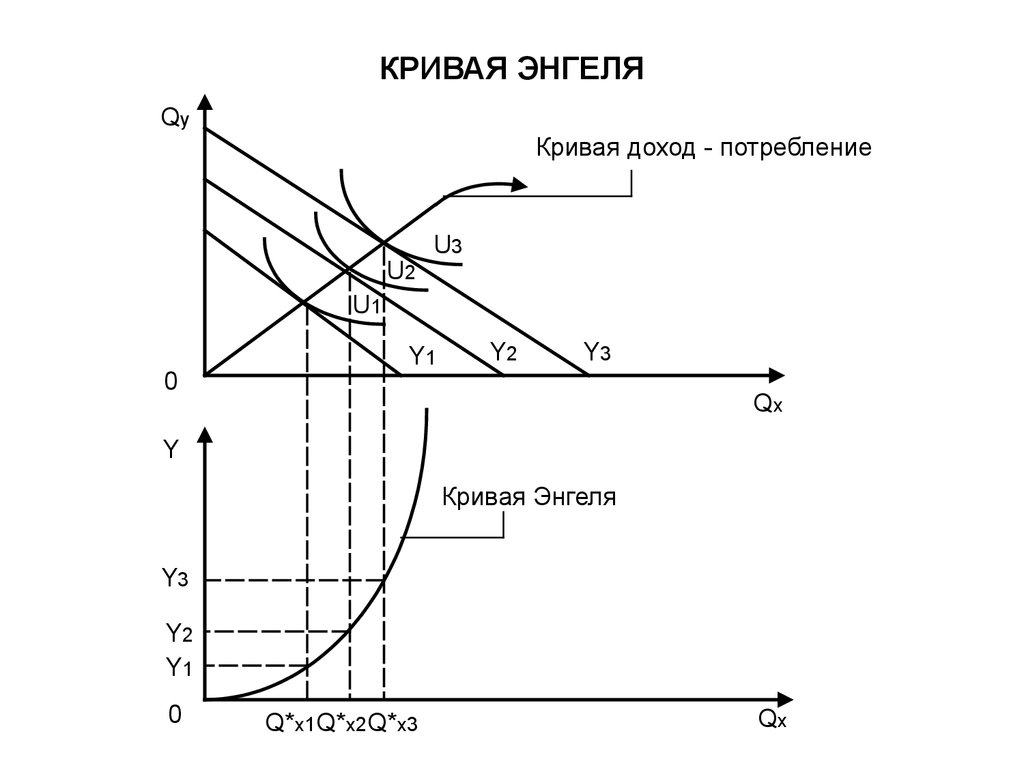
\includegraphics[width=0.7\textwidth]{КриваяЭнгеля}
	\end{figure}
	
	По виду кривой Энгеля можно судить о виде товара (роскоши или необходимый).
	\begin{figure}[h!]
		\centering
		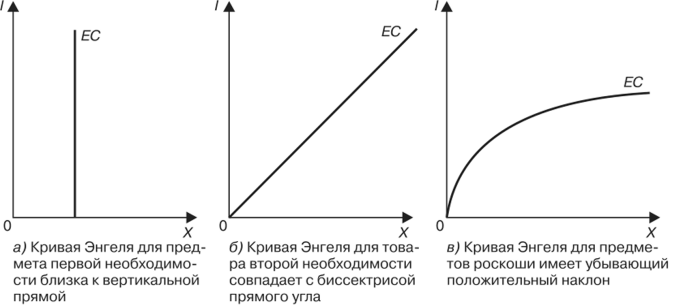
\includegraphics[width=0.8\textwidth]{ВидыКривыхЭнгеля}
	\end{figure}
	
	Таким образом, строятся две кривых Энгеля, для каждого товара в отдельности. Если же  построить кривую Энгеля в координатах $x$ и $y$ (двух товаров), то она будет выглядеть следующим образом.
	
	\begin{figure}[h!]
		\centering
		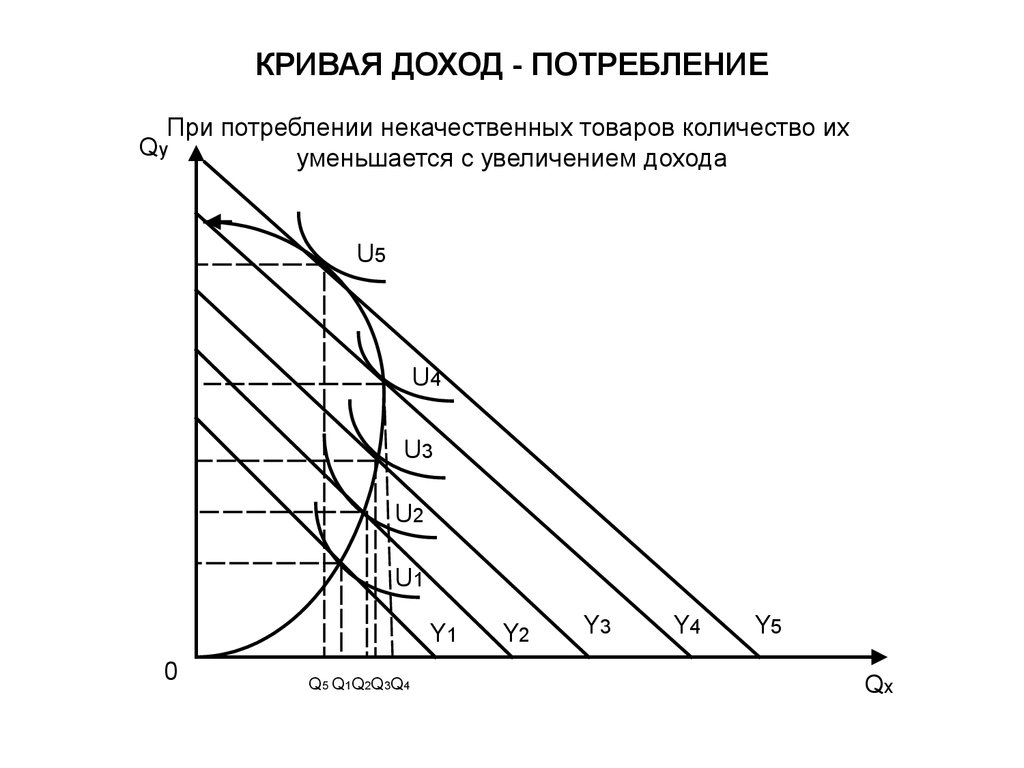
\includegraphics[width=0.7\textwidth]{КриваяЭнгеля2}
		\caption{при $E_x^m<0$} 
	\end{figure}
	
	\textbf{Эластичность по цене} -  показатель процентного изменения спроса какого-либо товара или услуги в результате изменения цены на этот товар.
	
	$$E_{x_i}^{p_i} = \dfrac{\sigma x_i}{\sigma p_i} \dfrac{p_i}{x_i}$$
	
	Если цена $p_{x_1}$ растет, то эластичность $E_{x_i}^{p_i} < 0$ (для товаров, которым мы можем найти замену). Также стоит обратить внимание на товары Гиффена, у которых при снижении цены на товар, будет снижаться и спрос, а эластичность при этом быть положительной (или же рост цены,  и рост спроса).
	\newpage
	
	\textbf{Перекрестная эластичность} -  показатель процентного изменения в количестве купленного товара или услуги в ответ на изменение в цене другого товара или услуги.
	
	$$E_{x_i}^{p_j} = \dfrac{\sigma x_i}{\sigma p_j} \dfrac{p_j}{x_i}$$
	
	Это товары субституты и комплименты. Если цена $p_{x_i}$ растет, и спрос на товар $j$ растет, то речь идет о взаимозаменяемых товаров($E_{x_i}^{p_j} > 0$). Если же цена на $i$-ый товар растет, а спрос на $j$-ый падает, то это взаимодополняемые товары. ($E_{x_i}^{p_i} < 0$)
	
	\subsection{Задача минимизации издержек при имеющемся уровне полезности}
	
	$$\min_{x,y \in\mathds{R}_{\geq 0}} p_x x + p_y y $$
	$$
	\text{s.t.}
	\begin{cases}
		U(x,y) \geq \bar{U}
	\end{cases}
	$$
	
	\bigskip
	
	\begin{exmp}
		$$\begin{cases}
			x\,p_x + y\,p_y &\rightarrow \min\\
			
			x^\alpha\,y^\beta& \geq \bar{U}
		\end{cases}$$
		
		$L(x,y)=-p_x x p_y y - \lambda (x^\alpha y^\beta - \bar{U})$
		
		$\begin{cases}
			L'_x=-p_x - \alpha x^{\alpha - 1} y^\beta \lambda =0\\
			
			L'_y=-p_y - \alpha y^{\beta - 1} x^\alpha \lambda =0
		\end{cases}$
		
		$\begin{cases}
			- \alpha x^{\alpha - 1} y^\beta \lambda = p_x\\
			
			- \alpha y^{\beta - 1} x^\alpha \lambda = p_y
		\end{cases}$\\ 
		
		Делим $L'_x$ на $L'_y$:
		
		$\dfrac{\alpha y}{\beta x} = \dfrac{p_x}{p_y}$
		
		$y=\dfrac{p_x}{p_y} \dfrac{\beta}{\alpha} x$\\
		
		Подставим в ограничение:
		
		$x^\alpha \cdot \left(\dfrac{p_x}{p_y} \dfrac{\beta}{\alpha} x \right)^\beta = \bar{U}$
		
		$x^{\alpha + \beta} = \dfrac{\bar{U}}{\left(\dfrac{p_x}{p_y} \dfrac{\beta}{\alpha} \right)^\beta}$\\
		
		Откуда:
		
		$$x^* = \bar{U}^{\dfrac{1}{\alpha + \beta}} \left(\dfrac{p_y}{p_x} \dfrac{\alpha}{\beta} \right)^{\dfrac{\beta}{\alpha + \beta}}$$  
		
		$$y^* = \bar{U}^{\dfrac{1}{\alpha + \beta}} \left(\dfrac{p_x}{p_y} \dfrac{\beta}{\alpha} \right)^{\dfrac{\alpha}{\alpha + \beta}}$$
				
		
	\end{exmp}
	
	\newpage
	
	\section{Лекция 4.}
	
	\subsection{Модели увеличения полезности и минимизации издержек}
	
	
	\begin{table}[h!] 
		
		\centering
		\begin{tabular}{c|c}
		
		 $ p_x x + p_y y \rightarrow \min\limits_{x,y \in\mathds{R}_{\geq 0}}$ & $ U(x,y)=x^\alpha y^\beta \rightarrow \max\limits_{x,y \in\mathds{R}_{\geq 0}} $ \\
		 
		$ \textbf{s.t.} \, x^\alpha y^\beta \geq \bar{U} $ & $ \textbf{s.t.} \, p_x x + p_y y \leq m $\\ \hline
		
		\\
		
		$ \begin{cases} 
			h_x(\textbf{p},\bar{U}) = \bar{U} \left( \dfrac{p_y}{p_x} \dfrac{\alpha}{\beta} \right)^\beta \\ 
			h_y(\textbf{p},\bar{U}) = \bar{U} \left( \dfrac{p_x}{p_y} \dfrac{\beta}{\alpha} \right)^\alpha
		\end{cases}
		$
		&
		$ \begin{cases} 
			x^* =  \dfrac{\alpha m}{p_x} \\ 
			y^* =  \dfrac{\beta m}{p_y} 
		\end{cases}
		$
		\\
		
		$\bar{U} \cdot \dfrac{p_x^\alpha p_y^\beta}{\alpha^\alpha \beta^\beta} = e^*$
		&
		$m \cdot \dfrac{\alpha^\alpha \beta^\beta}{p_x^\alpha p_y^\beta} = U(x^*,y^*) = V(\textbf{p},m)$
		\\
		
		&$U(x^*,y^*)$ -- косвенная функция полезности
		
		\end{tabular}
	
	\end{table}
	
	*При $\alpha + \beta = 1$
	
	Подставляем $V$ в $e^*$:
	
	$$e^* = m \cdot \dfrac{\alpha^\alpha \beta^\beta}{p_x^\alpha p_y^\beta} \dfrac{p_x^\alpha p_y^\beta}{\alpha^\alpha \beta^\beta} = m $$
	
	Так же равен и спрос
	
	$$x^* = \bar{U} \cdot \dfrac{p_x^\alpha p_y^\beta}{\alpha^\alpha \beta^\beta} \cdot \dfrac{\alpha}{p_x} = \bar{U} \left( \dfrac{p_y}{p_x} \dfrac{\alpha}{\beta} \right)^\beta$$
	
	Таким образом, когда $m = e$:
	
	$x(\textbf{p},m)=x(\textbf{p},e(\textbf{p},\bar{U})) = h_x (\textbf{p},\bar{U})$
	
	$h_x (\textbf{p},\bar{U}) = h_x(\textbf{p},V(\textbf{p},m)) = x(\textbf{p},m)$
	
	\subsection{Свойства функции спроса по Хиксу}
	
	$$e^* = \bar{U} \cdot \dfrac{p_x^\alpha p_y^\beta}{\alpha^\alpha \beta^\beta}$$
	
	$$h_x(\textbf{p},\bar{U}) = \bar{U} \left( \dfrac{p_y}{p_x} \dfrac{\alpha}{\beta} \right)^\beta$$ 
	
	\begin{itemize}
		\item Однородность нулевой степени по ценам\footnote{Однородность $k$ степени: $g(\gamma \textbf{x})=\gamma^k f(\textbf{x})$}
		
		$h_x(\gamma \textbf{x},\bar{U}) = \bar{U} \left(\dfrac{\gamma p_y \alpha}{\gamma p_x \beta} \right)y^\beta = \bar{U} \left(\dfrac{p_y \alpha}{p_x \beta} \right)y^\beta = h_x(\textbf{x},\bar{U})$ 
		\\
		 
		\item Лемма Шепарда 
		
		Частная производная функция расходов по конкретной цене равна конкретному спросу по Хиксу
		
		$$\dfrac{\delta e^*}{\delta p_x} = \bar{U} \left(\dfrac{\alpha p_y^\beta}{p_x^\beta \alpha^\alpha \beta^\beta} \right) = \bar{U} \left( \dfrac{p_y}{p_x} \dfrac{\alpha}{\beta} \right)^\beta = h_x(\textbf{p},\bar{U})$$ 
		
		\item Для спроса по Хиксу работает закон спроса
		
		$$\dfrac{\delta h_i}{\delta p_i} \leq 0$$ \\
		
		\textbf{Доказательство}
		
		$$\textbf{p} \, h(\textbf{p},\bar{U}) \rightarrow \min\limits_{x,y \in\mathds{R}_{\geq 0}}$$
		$$ \textbf{s.t.} \, U(h(\textbf{p}, \bar{U} )) \geq \bar{U} $$
		
		где $\textbf{p} = [p_1,p_2, \dots, p_n]$, $p_i \in\mathds{R}_{\geq 0}$ 
		
		и $h^*(\textbf{p},\bar{U})$ -- решение задачи\\
		
		Eсли же вектор цен: $\textbf{p} + \Delta = [p_1 + \Delta_1,p_2 + \Delta_2, \dots, p_n + \Delta_n]$
		
		$$(\textbf{p} + \Delta) \, h(\textbf{p} +\Delta,\bar{U}) \rightarrow \min\limits_{x,y \in\mathds{R}_{\geq 0}}$$
		$$ \textbf{s.t.} \, U(h(\textbf{p} +\Delta, \bar{U} )) \geq \bar{U} $$
		
		и решение задачи -- $h^*(\textbf{p} +\Delta,\bar{U})$\\
		
		$\Delta h = h^*(\textbf{p} +\Delta,\bar{U}) - h^*(\textbf{p},\bar{U})$
		
		Предположим, что цена на один товар возросла: $\Delta_i > 0, \Delta_{j \neq i} = 0$, и проанализируем издержки.
		
		$\textbf{p} \, h^*(\textbf{p},\bar{U}) \leq \textbf{p} \, h(\textbf{p},\bar{U}) \Rightarrow \textbf{p} h^*(\textbf{p},\bar{U}) \leq \textbf{p}\, h^*(\textbf{p} + \Delta,\bar{U})$
		
		$(\textbf{p}+\Delta) \, h^*(\textbf{p}+\Delta,\bar{U}) \leq (\textbf{p}+\Delta) \, h(\textbf{p}+\Delta,\bar{U}) \Rightarrow (\textbf{p}+\Delta) h^*(\textbf{p}+\Delta,\bar{U}) \leq (\textbf{p}+\Delta) \, h(\textbf{p},\bar{U})$
		
		Откуда
		
		$$
		\text{s.t.}
		\begin{cases}
			\textbf{p}h^*(\textbf{p},\bar{U}) \leq \textbf{p} h^*(\textbf{p} + \Delta,\bar{U})\\
			
			(\textbf{p}+\Delta) h^*(\textbf{p}+\Delta,\bar{U}) \leq (\textbf{p}+\Delta) h(\textbf{p},\bar{U})
		\end{cases}
		$$
		
		Сложим два неравенства
		
		$\textbf{p}h^*(\textbf{p},\bar{U}) + (\textbf{p}+\Delta) \, h^*(\textbf{p}+\Delta,\bar{U}) \leq \textbf{p} \, h^*(\textbf{p} + \Delta,\bar{U}) + (\textbf{p}+\Delta) \, h(\textbf{p},\bar{U})$
		
		$\textbf{p} (h^*(\textbf{p},\bar{U}) - h^*(\textbf{p} + \Delta,\bar{U})) - (\textbf{p}+\Delta) (h(\textbf{p},\bar{U}) - h^*(\textbf{p}+\Delta,\bar{U})) \leq 0$
		
		$- \Delta (h(\textbf{p},\bar{U}) - h^*(\textbf{p}+\Delta,\bar{U})) \leq 0$
		
		Отсюда следует $h_i(\textbf{p},\bar{U}) \geq h_i^*(\textbf{p}+\Delta,\bar{U})$
	\end{itemize}
	
	
	\newpage
	
	\section{Лекция 5.}
	
	\subsection{Задачки}
	
	\begin{exc}
		$$x p_x+y p_y \rightarrow \min\limits_{x,y,\geq 0}$$
		
		$$
		\text{s.t.}
		\begin{cases}
			\min\{\alpha x,y\} \geq \bar{U}
		\end{cases}
		$$
		
		$\alpha x = y = \bar{U}$
		
		$x^* = \dfrac{\bar{U}}{\alpha}$
		
		$y^* = \bar{U}$
		
		$e(p_x,p_y,h_1(\textbf{p},\bar{U}),h_2(\textbf{p},\bar{U})) = p_x \frac{\bar{U}}{\alpha} + p_y \bar{U} = \bar{U}(\dfrac{p_x}{\alpha} + p_y)$
	\end{exc}

	\begin{exc}
		$$\min\{\alpha x,y\} \rightarrow \max\limits_{x,y,\geq 0}$$
		
		$$
		\text{s.t.}
		\begin{cases}
			x p_x+y p_y \leq m
		\end{cases}
		$$
		
		$x^* = \dfrac{m}{p_x + \alpha p_y}$
		
		$y^* = \dfrac{\alpha m}{p_x + \alpha p_y}$
		
		$ u(x^*,y^*)=\min\{\dfrac{m}{p_x + \alpha p_y},\dfrac{\alpha m}{p_x + \alpha p_y}\} = \dfrac{m}{p_x + \alpha p_y}$
	\end{exc}
	
	\subsection{Эффект дохода и эффект замещения}
	
	\begin{figure}[h!]
		\centering
		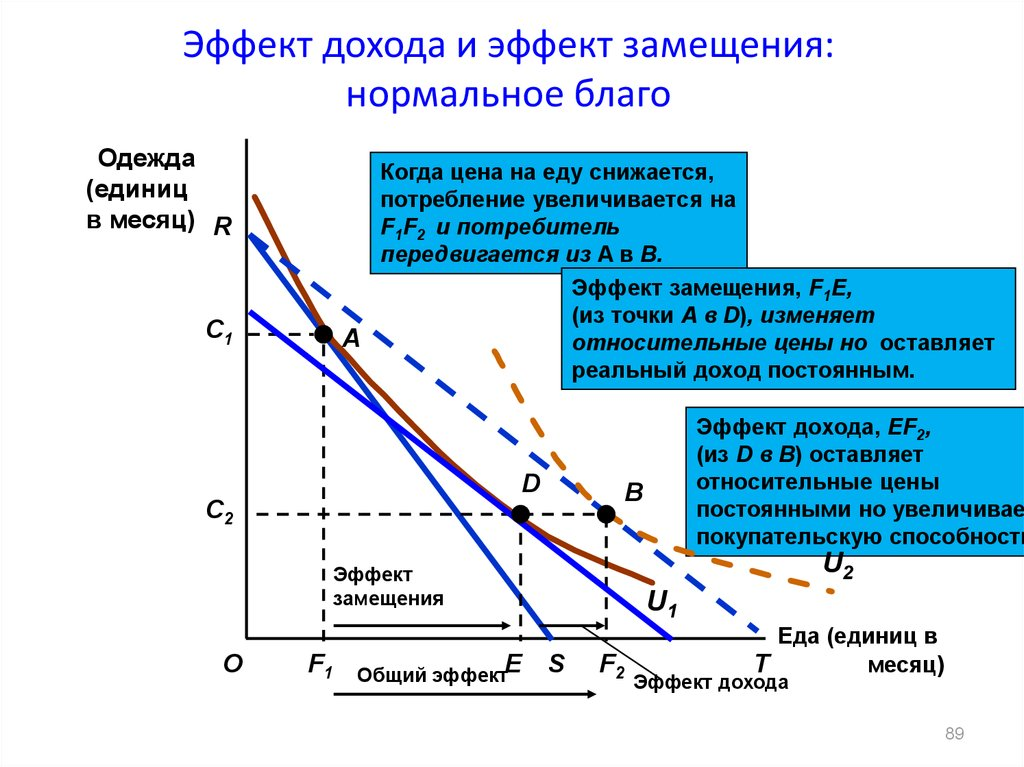
\includegraphics[width=0.65\textwidth]{ЭффектДоходаИЗамещения}
	\end{figure}

	\begin{exmp}
		
		$x=10+\dfrac{m}{10 p_1}$; $m=120$; $p_1 =3$
		
		$X_1 = 10 + \dfrac{120}{10 \cdot 3} = 14$
		
		При снижении цены $p_1 = 2$. Таким образом теперь потребление составит $X_2 =10+\dfrac{120}{10 \cdot 2} = 16$.
		
		Но существует промежуточный уровень, который называется эффектом замены.
		
		Цена снизилась, но мы хотим оставить прошлый набор благ, для этого нам необходимо изменить наш доход. $\Delta m = m' - m = X_1 p'_1 - X_1 p_1 = X_1 (p'_1 - p_1) = -14$. То есть наш доход теперь будет $m' = 120 - 14 = 106$, а потребление $X_3 = 10 + \dfrac{106}{2 \cdot 10} = 15.3$. Эффект замещения $15.3-14=1.3$.
		
		*$\Delta m$ - компенсационная вариация по Слуцкому(на рисунке $A A_1$), т.е. доход отнимается или добавляется в той мере, в какой новый уровень денежного дохода может обеспечить прежний набор благ. 
		
		**В модели Хикса (компенсационная вариация по Хиксу) компенсирующий доход позволяет потребителю после изменения цен сохранить прежний уровень удовлетворенности (при другом по структуре товарном наборе на той же кривой безразличия).
		
		Эффект замещения (на рисунке $X_1 X_3$) говорит о том, что так как цена на первый товар упала, потребитель начинает покупать этого товара больше, но за счет снижения потребления второго товара. 
		
		Но так как доход на самом деле остается на одном месте, существует эффект дохода (на рисунке $X_3 X_2$). $16-15.3=0.7$
		
	\end{exmp}
	
	
\end{document}


% Examples and Shortcuts

\begin{defi}
	Определение чего-то
\end{defi}


\begin{thm}
	
\end{thm}	


\begin{coll}
	
\end{coll}	


\begin{nb}
	
\end{nb}	


\begin{nb}
	
\end{nb}	


\begin{exmp}
	
\end{exmp}	


\begin{tikzcd}
	A \arrow[rd] \arrow[r, "\phi"] 
	&B \\
	& C \arrow[u]
\end{tikzcd}

% Пример мат. постановки

$$\text{min} \quad \sum\limits_{e \in E} x_e$$

$$
\text{s.t.}
\begin{cases}
	\sum\limits_{e \in E_v} x_e \geq 1& \forall v \in V\\
	x \in \{0, 1\}^{|E|} &
\end{cases}
$$

% Пример алгоритма

\begin{algorithm}[H]
	\SetAlgoLined
	\SetKwFunction{FDFS}{DFS}
	\SetKwProg{Fn}{Function}{:}{}
	\Fn{\FDFS{$u$}}{
		$VisitFunc(u)$\;
		$visited[u] = True$\;
		\For{$w \in \text{adj}[u]$}
		{
			\If{$visited[w] = False$}
			{
				$FoundFunc(w)$\;
				$\text{DFS}(w)$\;
			}						
		}
		$OutFunc(u)$\;
	}
	
	DFS(start)
	\caption{Depth-first search}
\end{algorithm}
